 \begin{figure}[H]
     \centering
     \includegraphics[width=\textwidth]{figures/ch_design/controller/ControlDiagram.png}
     \caption{Block diagram illustration of the control system  to control the levitation of the Quadcopter.}
     \label{fig:controlDiagram}
 \end{figure}

To avoid steady state error, it is necessary to examine PID controller, which stands for proportional integrate derivative controller. In the following sections there will be an explanation of PID controller, and afterwards there will be a section of what have been chosen for this project.  


\section{PID controller} % ???Different Controller
% her skal der skrives om de forskellige kontrollers (p-, pd-, pi-, pid-controller) og vaglet af vores kontroller
\begin{figure}[H]
    \centering
    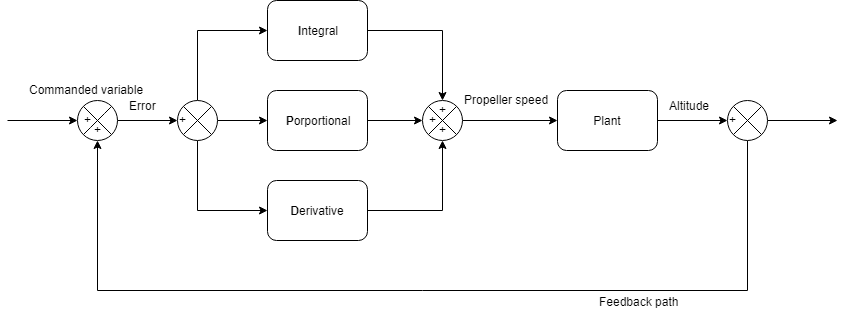
\includegraphics[width=0.9\textwidth]{figures/ch_design/PIDControl.png}
    \caption{PID control system}
    \label{fig:PID_Controller}
\end{figure}
The above block diagram illustrates how a PID control system looks like. The block diagram will used for explanations of P, PI and PID control. In this section there will be different block diagram for each control.

\begin{figure}[H]
    \centering
    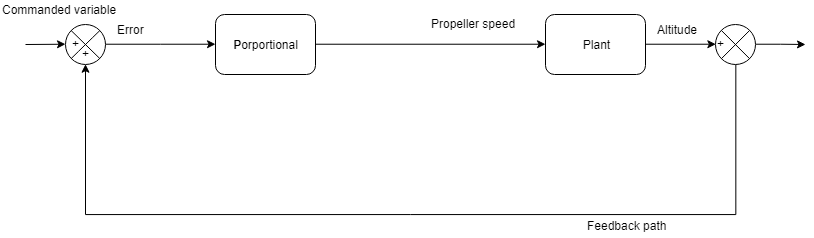
\includegraphics[width=0.8\textwidth]{figures/ch_design/PControl.png}
    \caption{Proportional control system}
    \label{fig:P_Control}
    \end{figure}
Proportional control Is used to decrease the steady state error. An example would be If we want a drone to rise to an altitude of 50 meter, the set point which in the block diagram is commanded variable, will be set to 50 meters. At the current time the output is 0 meter since the drone haven’t done anything yet. However, when the drone rises to around 50 meters, it will decrease the propeller speed, and increases when it’s under 50 meters and will continue this way. The following graph \ref{gra:P_Control_graph} will illustrate the example. 
\begin{figure}[H]
    \centering
    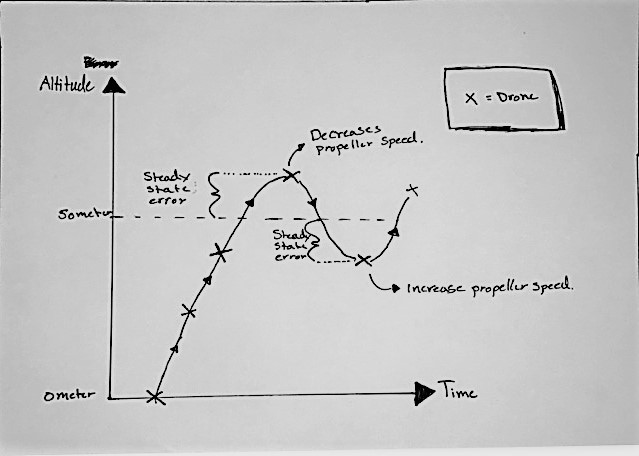
\includegraphics[width=0.8\textwidth]{figures/ch_design/PGraph.jpg}
    \caption{Proportional control graph}
    \label{gra:P_Control_graph}
    \end{figure}
Despite reduction of steady state error, proportional controller can never mange to eliminate the steady state error of the above graph. However, the proportional the main function is to introduce a gain that is proportional to the error, which is produced by comparing the system’s input and output.



\section{Design of proportional controller}\label{sec:design_controller}
As it has been decided to use a proportional controller to regulate the system, the proportional gain $K_P$ has to be found. 
When finding the value of $K_P$ the requirements from chapter \ref{ch:Req} have to be taken into consideration. 
The requirements that have to be taken into consideration are:
\begin{itemize}
    \item Overshoot of max 30\%
    \item Settling time of  max 10 seconds
    \item Steady state of $\pm$5\%
\end{itemize}
To find $K_P$ we have to start finding the damping factor. From the allowed overshoot the damping ratio $\zeta$ can be found with the formula:
\begin{equation}
    \zeta = \frac{-\ln(overshoot/100)}{\sqrt{\pi^2+\ln(overshoot/100)}}
\end{equation}
With a overshoot of 30\% the damping ratio are found to be 0.409, and from this ratio the phase margin $\Phi_M$ can then be found with the use of the formula:
\begin{equation}
    \Phi_M = \arctan\left(\frac{2\zeta}{\sqrt{-2\zeta^2+\sqrt{1+4\zeta^4}}}\right)
\end{equation}
The phase margin is calculated to % ??? find den rigtige beregning